% !TEX encoding = UTF-8 Unicode
\documentclass[
10pt,
aspectratio=169,
]{beamer}
\setbeamercovered{transparent=10}
\usetheme[
%  showheader,
%  red,
  purple,
%  gray,
%  graytitle,
  colorblocks,
%  noframetitlerule,
]{Verona}

\usepackage[T1]{fontenc}
\usepackage[utf8]{inputenc}
\usepackage{lipsum}
%%%%%%%%%%%%%%%%%%%%%%%%%%%%%%%
% Mac上使用如下命令声明隶书字体,windows也有相关方式,大家可自行修改
%\providecommand{\lishu}{\CJKfamily{zhli}}
%%%%%%%%%%%%%%%%%%%%%%%%%%%%%%%
\usepackage{tikz}
\usetikzlibrary{shapes,snakes}
\usetikzlibrary{fadings}
%
%\setbeamertemplate{sections/subsections in toc}[ball]
%\usepackage{xeCJK}
\usepackage{listings}
\usepackage{caption}
\usepackage{subcaption}
\usefonttheme{professionalfonts}
\def\mathfamilydefault{\rmdefault}
\usepackage{amsmath}
\usepackage{multirow}
\usepackage{booktabs}
\usepackage{bm}
\setbeamertemplate{section in toc}{\hspace*{1em}\inserttocsectionnumber.~\inserttocsection\par}
\setbeamertemplate{subsection in toc}{\hspace*{2em}\inserttocsectionnumber.\inserttocsubsectionnumber.~\inserttocsubsection\par}
\setbeamerfont{subsection in toc}{size=\small}
\AtBeginSection[]{%
	\begin{frame}%
		\frametitle{Outline}%
		\textbf{\tableofcontents[currentsection]} %
	\end{frame}%
}

\AtBeginSubsection[]{%
	\begin{frame}%
		\frametitle{Outline}%
		\textbf{\tableofcontents[currentsection, currentsubsection]} %
	\end{frame}%
}

\title{Introducci\'on a Python}
\subtitle{Comandos b\'asicos y gr\'aficas en Python}
\author[L.M.]{Luis Alejandro Morales, Ph.D.}
\mail{lmoralesm@unal.edu.co}
\institute[UNAL]{Facultad de Ingenier\'ia\\
Universidad Nacional de Colombia}
\date{\today}
\titlegraphic[width=3cm]{logo_01u}{}

%%%%%%%%%%%%%%%%%%%%%%%%%%%%%%%%
% ----------- 标题页 ------------
%%%%%%%%%%%%%%%%%%%%%%%%%%%%%%%%
% New commands
\newcommand{\gi}{\texttt{Git}}
\newcommand{\gih}{\texttt{GitHub}}
%\newcommand{\co}[1]{\alert{\textbf{\large \texttt{#1}}}}
\newcommand{\co}[1]{\alert{\textbf{\texttt{#1}}}}

\tikzset{
    *|/.style={
        to path={
            (perpendicular cs: horizontal line through={(\tikztostart)},
                                 vertical line through={(\tikztotarget)})
            % is the same as (\tikztostart -| \tikztotarget)
            % but just to be safe: http://tex.stackexchange.com/a/29781/16595
            -- (\tikztotarget) \tikztonodes
        }
    }
}
\begin{document}



\maketitle

%%% define code
\defverbatim[colored]\lstI{
	\begin{lstlisting}[language=C++,basicstyle=\ttfamily,keywordstyle=\color{red}]
	int main() {
	// Define variables at the beginning
	// of the block, as in C:
	CStash intStash, stringStash;
	int i;
	char* cp;
	ifstream in;
	string line;
	[...]
	\end{lstlisting}
}
%%%%%%%%%%%%%%%%%%%%%%%%%%%%%%%%
% ----------- FRAME ------------
%%%%%%%%%%%%%%%%%%%%%%%%%%%%%%%%

%---
\section{Generalidades}
\begin{frame}[c]{?`Que es Python?}
Python es un \alert{lenguaje de programación interpretado}, \alert{orientado a objetos}, de \alert{ alto nivel} y con \alert{semántica dinámica}. Sus estructuras de datos integradas de alto nivel, combinadas con escritura dinámica y enlace dinámico, lo hacen muy atractivo para el \alert{desarrollo rápido de aplicaciones}, así como para su uso como \alert{lenguaje de secuencias de comandos} o  para \alert{conectar componentes existentes}. La \alert{sintaxis simple y fácil} de aprender de Python enfatiza la legibilidad y, por lo tanto, reduce el costo de mantenimiento del programa. Python admite \alert{módulos y paquetes}, lo que fomenta la \alert{modularidad} del programa y la reutilización del código. El intérprete de Python y la extensa biblioteca estándar están disponibles en formato fuente o binario sin costo para todas las plataformas principales y se pueden distribuir \alert{gratuitamente}.
\end{frame}

\begin{frame}[c]{?`Como se ejecuta python en su computador?}
\begin{columns}
\column{0.5\textwidth}
\centering
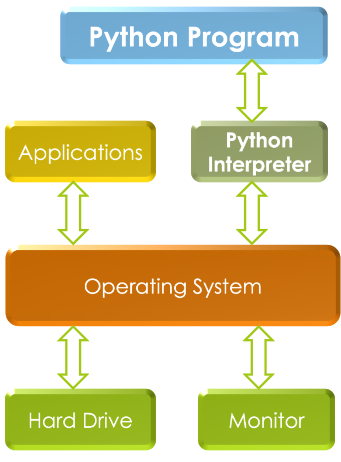
\includegraphics[width=0.75\textwidth]{fig1.png}
\column{0.6\textwidth}
\begin{itemize}
\item Python programs no se ejecutan directamente en el sistema opertativo (OS).
\item Otro programa llamado \alert{interprete} o \alert{m\'aquina virtual} toma el programa y lo pasa (ejecuci\'on) a lenguage de maquina (entendido por el OS).
\item Aqui se escribiran programas ejecutados por el interprete.
\end{itemize}
\end{columns}
\end{frame}

\begin{frame}[c]{?`Que tipo de lenguage es Python?}
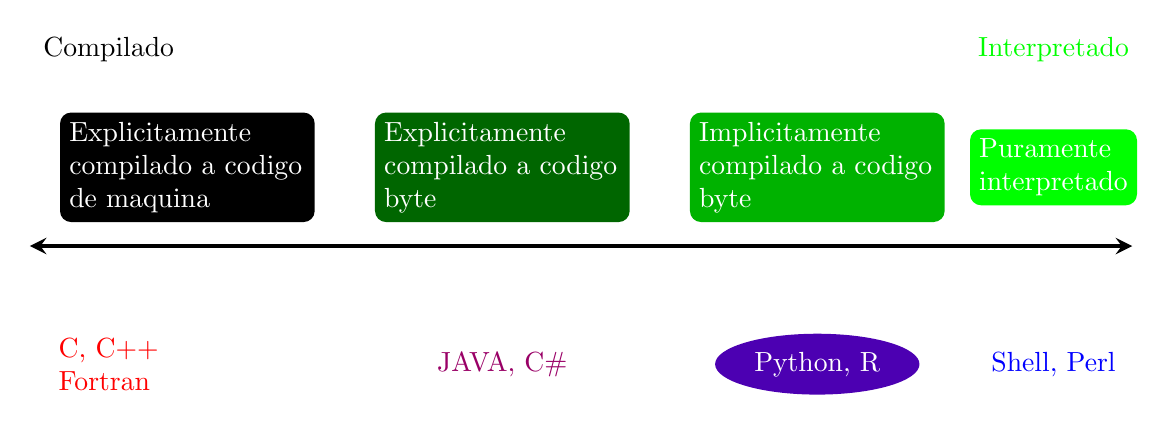
\begin{tikzpicture}
\node[text=black] at (-2,2.5) {Compilado};
\node[rounded corners,text width=3cm,fill=black,text=white] at (-1,1) {Explicitamente compilado a codigo de maquina};
\node[rounded corners,text width=3cm,fill=black!60!green,text=white] at (3,1) {Explicitamente compilado a codigo byte};
\node[rounded corners,text width=3cm,fill=black!30!green,text=white] at (7,1) {Implicitamente compilado a codigo byte};
\node[rounded corners,align=left,fill=green,text=white] at (10,1) {Puramente\\ interpretado};
\node[text=green] at (10,2.5) {Interpretado};
\draw [stealth-stealth, ultra thick](-3,0) -- (11,0);
\node[text=red,align=left] at (-2,-1.5) {C, C++\\ Fortran};
\node[text=red!60!blue] at (3,-1.5) {JAVA, C\#};
\node[ellipse,fill=red!30!blue, text=white] at (7,-1.5) {Python, R};
\node[text=blue] at (10,-1.5) {Shell, Perl};
\end{tikzpicture}
\end{frame}


\begin{frame}[c]{?`Para que sirve Python y sus ventajas?}
Untilidades de Python
\begin{itemize}
\item Science: Deterministic and statistical modelling
\item Instrumental control
\item Embedded systems
\item Web services
\item On-line games
\end{itemize}
Ventajas de Python
\begin{itemize}
\item Relativamente facil de aprender
\item Gran numero de librerias
\item Versatil e independiente de la plataforma
\item Comunidad con fuerte soporte
\end{itemize}
\end{frame}


\begin{frame}[c]{?`Como instalar Python?}
\begin{itemize}
\item Python tiene dos versiones:
\begin{itemize}
\item 2.x: Version m\'as antigua, carece de mantenimiento.
\item 3.x; Version reciente, con suporte actual. 
\end{itemize}
\item Minimo hardware requerido: $>$ 4GB de RAM, $>5$ GB de disco duro libre (para la instalaci\'on de librerias se requier m\'as espacio)
\end{itemize}
\begin{itemize}
\item Unix/Linux y Mac OS, Python viene instalado por defecto,:)

\item MS Windows
\begin{itemize}
\item Descargar el installador de Python en (\href{https://www.python.org/downloads/windows/}{https://www.python.org/downloads/windows/})
\item Ejecutar el installador \co{pytho3.x.x.exe}
\item Personalizar la instalaci\'on
\item Installar Python
\item Verificar la installaci\'on: Busque \co{cmd} y escriba \co{python --version}
\end{itemize}
\end{itemize}
\end{frame}

\begin{frame}[c]{?`Como usar Python?}
\begin{enumerate}
\item Ejecutar comandos y codigos directamente desde el interprete de Python

\begin{enumerate}
\item Abra la termninal (busque \co{cmd})
\item Ejecute \co{python3} o \co{python}. Producir\'a:
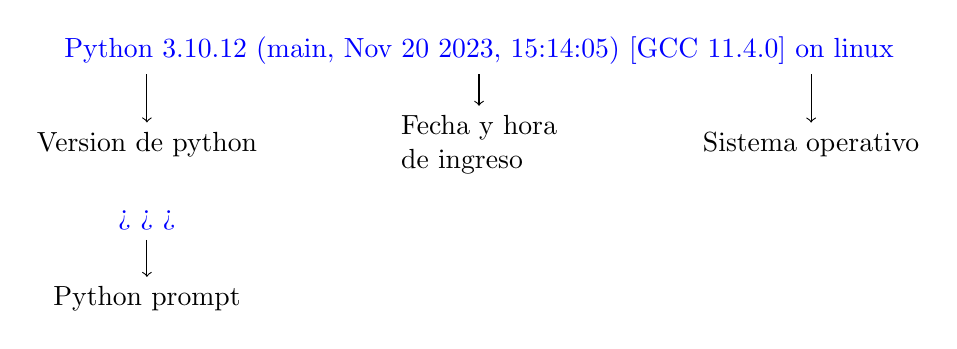
\begin{tikzpicture}[node distance=12em]
\node(G) [text=blue] {Python 3.10.12 (main, Nov 20 2023, 15:14:05) [GCC 11.4.0] on linux};
\node(H)  [align=left] [below=0.7cm] {Fecha y hora\\ de ingreso};
\node(H1) [left of=H]  {Version de python};
\node(H2) [right of=H] {Sistema operativo};
\draw[->,*|] (G.south) to     (H1.north);
\draw[->]    (G.south) --     (H.north);
\draw[->]    (G.south) to[*|] (H2.north);
\node(F) [text=blue,below of=H1, below=-3.5cm] {> > >};
\node(F1) [below of=F,below=-3.5cm] {Python prompt};
\draw[->,*|] (F.south) to     (F1.north);
\end{tikzpicture}
\end{enumerate}
\item Correr programas escritos en un archivo (e.g. \co{myprogram.py})
\begin{enumerate}
\item Abra la termninal (busque \co{cmd})
\item Para ejecutar el programa: \co{python3 myprogram.py} o \co{python myprogram.py}
\end{enumerate}

\end{enumerate}

\end{frame}



%---
\section{Comandos b\'asicos en Python}
\begin{frame}[c]{Tipos de datos en Python}
\end{frame}

\begin{frame}[c]{Objetos en Python}
\end{frame}

\begin{frame}[c]{Condicionales en Python}
\end{frame}

\begin{frame}[c]{Loops en Python}
\end{frame}

\begin{frame}[c]{Leer datos externos}
\end{frame}

\begin{frame}[c]{Imprimir datos en Python}
\end{frame}

%---
\section{Graficas en Python}
\begin{frame}[c]{Paquetes}
\end{frame}

\begin{frame}[c]{Graficar datos}
\end{frame}

\begin{frame}[c]{Atributos de las graficas}
\end{frame}

\begin{frame}[c]{Multiples axes en una grafica}
\end{frame}




`



%\begin{frame}[c]{?`Que es \gi?}
%\begin{columns}
%\column{0.6\textwidth}
%\large{
%\begin{block}{\gi}
%\begin{itemize}
%    \item \gi\ es un programa/sistema usado para el control de versiones en proyectos, particularmente, en c\'odigos de computador.
%    \item \gi\ fue inventado en 2005 por Linus Torvalds, creador de \texttt{Linux}, con el fin de manejar proyectos grandes multiusuario (e.g. kernel de \texttt{Linux} escrito en \texttt{C}) de manera eficiente y r\'apida.
%    \item Git est\'a escrito en \texttt{C} y viene por defecto en \texttt{Linux}. Puede ser instalado en \texttt{MS Windows}.
%\end{itemize}
%\end{block}
%}
%\column{0.4\textwidth}
%\begin{center}
% %\begin{figure}
% \includegraphics[width=\textwidth]{linus.jpeg}
% %\vspace{-0.5cm}
% %\caption{\tiny Fuente: https://en.wikipedia.org/wiki}
% %\end{figure}
% \end{center}
%\end{columns}
%\end{frame}	
%%---
%\section{?`Para que sirve \gi?}
%\begin{frame}[c]{?`Para que sirve \gi?}
%%\begin{columns}
%%\column{0.6\textwidth}
%\large{
%\begin{block}{Utilidades de \gi}
%\begin{itemize}
%    \item Trabajo en grandes proyectos con colaboracion de multiples usuarios y servidores.
%    \item Control de cambios lo que permite ir a hacia adelante o hacia atras en la historia del proyecto.
%    \item Sistema distribuido lo que permite que multiples usuarios hagan cambios y sean a la vez servidores del proyecto.
%\end{itemize}
%\end{block}
%}
%\end{frame}	
%
%\begin{frame}[c]{Modelo centralizado Vs \alert{modelo distribuido}}
%\vspace{-0.2cm}
%\begin{center}
% \includegraphics[width=0.87\textwidth]{dist.png}
% \end{center}
%\end{frame}	
%%---
%\section{Tratamiento de cambios en un repositorio en \gi}
%\begin{frame}[c]{Proyecto local en \gi}
%\vspace{-0.2cm}
%\begin{center}
% %\begin{figure}
% \includegraphics[width=0.55\textwidth]{gitp.png}
% %\vspace{-0.5cm}
% %\caption{\tiny Fuente: https://en.wikipedia.org/wiki}
% %\end{figure}
% \end{center}
%%\end{columns}
%\end{frame}	
%
%\begin{frame}[c]{Ciclo de vida de un archivo de un repositorio en \gi}
%%\column{0.4\textwidth}
%\begin{center}
% %\begin{figure}
% \includegraphics[width=0.8\textwidth]{gitf.png}
% %\vspace{-0.5cm}
% %\caption{\tiny Fuente: https://en.wikipedia.org/wiki}
% %\end{figure}
% \end{center}
%%\end{columns}
%\end{frame}	
%
%%---
%\section{\gih}
%\begin{frame}[c]{\gih}
%\begin{columns}
%\column{0.8\textwidth}
%\begin{block}{\gih}
%\begin{itemize}
%    \item \href{http://www.github.com}{\gih} es una p\'agina web de libre acceso para archivar repositorios online.
%    \item Muchos repositorios de codigo abierto como el kernel de Linux usan \gih.
%    \item ?`Es necesario tener \gih\ para usar \gi? \textbf{No!}
%    \begin{itemize}
%        \item Se puede usar \gi\ localmente, o  
%        \item se puede configurar un servidor para compartir archivos.
%    \end{itemize}     
%\end{itemize}
%\end{block}
%\column{0.2\textwidth}
%\begin{center}
% \includegraphics[width=0.8\textwidth]{ghub.png}
% \end{center}
%\end{columns}
%\end{frame}
%
%
%%---
%\section{Commandos b\'asicos en \gi}
%\begin{frame}[c]{Workflow b\'asico en \gi}
%\begin{block}{Workflow b\'asico en \gi}
%\begin{enumerate}
%    \item \alert{Pull} el directorio \gi\ del servidor remoto (opcional).
%    \item \alert{Modificar} los archivos en el directorio de trabajo
%    \item \alert{Stage} archivos. Adicionar un copia del archivo a la staging area.
%    \item Hacer un \alert{commit}, el cual toma los archivos en la staging area y archiva la copia en el directorio de \gi. 
%    \item \alert{Push} el directorio \gi\ a el servidor remoto (opcional).
%\end{enumerate}
%\end{block}
%\begin{center}
% \includegraphics[width=\textwidth]{workflow.png}
%\end{center}
%\end{frame}	
%
%\begin{frame}[c]{Configuraci\'on inicial en \gi}
%\begin{block}{Alistarse para usar \gi}
%    \begin{enumerate}
%    \item Introducir \texttt{username} y \texttt{email} para ser usado por \gi\ cuando se haga un \texttt{commit}.\\
%     \co{\$ git config --global user.name “Luis Morales”}\\ %\vspace{0.3cm}
%     \co{\$ git config --global user.email lmoralesm@unal.edu.co}
%     \begin{itemize}
%         \item Para verificar la configuraci\'on:\\
%              \co{\$ git config -list}
%         \item Esta configuraci\'on es para todos los proyectos \gi.
%         \item La configuraci\'on anterior puede ser para un proyecto determinado si no se usa la opci\'on \co{-{}-global}
%         \item Adem\'as en la configuraci\'on inicial se puede escoger el editor para escribir mensajes en commit:
%         \co{\$ git config -{}-global core.editor vim}
%     \end{itemize}
%    \end{enumerate}
%\end{block}
%\end{frame}	
%
%\begin{frame}[c]{Crear una copia local del repositorio}
%\begin{block}{Crear copia local del repositorio \gi}
%\begin{enumerate}
%    \item Dos escenarios posibles:
%    \begin{enumerate}
%        \item Clonar un repositorio existente en su directorio local:\\
%        \co{\$ git clone <url> [local\_dir\_name]}\\
%        Crea el directorio \texttt{local\_dir\_name}, el cual contiene una copia de los archivos del repo original, y un directorio \texttt{.git}.
%        \item Crear un repositorio \gi\ en el directorio actual:\\
%        \co{\$ git init}\\
%        Crea el directorio \texttt{.git} en el directorio actual.  
%    \end{enumerate}
%\end{enumerate}
%\end{block}
%\end{frame}	
%
%\begin{frame}[c]{Commit archivos}
%\begin{block}{Commit archivos en el repo local}
%\begin{enumerate}
%    \item Una ves creado el directorio, se puede:
%    \begin{enumerate}
%        \item Se pueden crear archivos dentro del repositorio y adicionarlos a la staging \'area: \\
%        \co{\$ git add README.md file1.c}\\
%        Toma un snapshop de estos archivos en este instante de tiempo y los adiciona a la staging \'area.
%        \item Commit cambios en el repo (mover los staged cambios al repo)
%        \co{\$ git commit -m "initial project version"}\\
%    \end{enumerate}
%    Para unstage cambios (deshacer cambios) en un archivo antes de commit este):\\
%    \co{\$ git reset HEAD -{}- filename}
%    Para deshacer cambios en un archivo despu\'es de commit este:\\
%    \co{\$ git checkout -{}- filename}
%\end{enumerate}
%\end{block}
%\end{frame}	
%
%\begin{frame}[c]{Status y Diff}
%\begin{block}{Status y Diff}
%\begin{itemize}
%    \item Para mirar el \texttt{status} de los archivos en el directorio de trabajo o repo y la staging area:\\
%    \co{\$ git status} o \\
%    \co{\$ git status -s}\\
%    donde la opci\'on \co{-s} muestra una versi\'on del archivo en la staging \'area.
%    \item Para ver cual archivo ha sido modificado pero no est\'a en la staging \'area:\\
%    \co{\$ git diff}
%    \item Para ver cambios que ya estan en la staging \'area:\\
%    \co{\$ git diff}
%\end{itemize}
%\end{block}
%\end{frame}	
%
%\begin{frame}[c]{Chequeando los \texttt{logs}}
%\begin{block}{Chequeando los \texttt{logs}}
%\texttt{log} es un comando en \gi\ que permite conocer los cambios hechos en el repo. Algunos comandos importantes:
%\begin{itemize}
%    \item Chequeando la versi\'on larga de \texttt{logs}:\\
%    \co{\$ git log}
%    \item Chequeando la versi\'on larga de \texttt{logs}:\\
%    \co{\$ git log -{}-oneline}
%    %\begin{center}
%    %\includegraphics[width=\textwidth]{}
%    %\end{center}
%    \item Para mostrar los 5 m\'as recientes cambios:\\
%    \co{\$ git log -5}
%\end{itemize}
%Notas:
%\begin{enumerate}
%    \item Los cambios son listado de acuerdo con el commitID \#.
%    \item Todos los cambios hechos en el repo antes de haber sido clonado o jalado estan incluidos en \texttt{logs}.  
%\end{enumerate}
%\end{block}
%\end{frame}	
%
%\begin{frame}[c]{Pulling y pushing}
%\begin{block}{Pulling y pushing}
%\texttt{pull} y \texttt{push} son dos comandos que permiten jalar el repo de un servidor externo y enviar cambios a el repo, respectivamente. Buenas pr\'acticas en el uso de estos comandos son:
%\begin{enumerate}
%    \item \texttt{Add} y \texttt{commit} los cambios al repo local.
%    \item \texttt{pull} del repo remoto para obtener los cambios mas recientes. En caso de conflictos, \texttt{add} y \texttt{commit} estos al repo. 
%    \item \texttt{push} los cambios al repo remoto.
%\end{enumerate}
%Para incluir los cambios m\'as recientes del repo remoto en el repo local:\\
%\begin{enumerate}
%    \item Para bajar el contenido del repo remoto al repo local (optional):\\
%    \co{\$ git fetch}
%    \item Para bajar el contenido del repo remoto y actualizar el repo local:\\
%    \co{\$ git pull origin master}\\
%\end{enumerate}
%Para \texttt{push} los cambios realizados en el repo local a el repo remoto:\\
%\co{\$ git push origin master}
%\end{block}
%\end{frame}	
%
%\begin{frame}[c]{Branching}
%\vspace{-0.3cm}
%\begin{block}{Branching}
%\texttt{branch} es un comando que permite crear ramificaciones dentro del repo local para hacer cambios experimentales en el.
%\begin{itemize}
%    \item Para crear un \texttt{branch} llamado e.g. experiment1:\\
%    \co{\$ git branch experiment1}
%    \item Para listar todos los branches en el repo:\\
%    \co{\$ git branch}\\
%    Note que * indica el branch actual
%    \item Para cambiar al branch \texttt{experiment1}:\\
%    \co{\$ git checkout experiment1}
%    \item Para introducir los cambios hechos en  \texttt{experiment1} dentro del branch \texttt{master}:\\
%    \co{\$ git checkout master}\\
%    \co{\$ git merge experiment1}      
%\end{itemize}
%Notas:
%\begin{enumerate}
%    \item \co{\$ git log -{}-graph} puede ser usado para mostrar los branches gr\'aficamente. 
%    \item Los branches est\'an solo en el repo local.
%\end{enumerate}
%\end{block}
%\end{frame}	
%
%\begin{frame}[c]{Resumen}
%\vspace{-0.2cm}
%\begin{block}{Resumen}
%Configuraci\'on inicial y clonaci\'on
%\begin{enumerate}
%    \item \co{\$ git config -{}-global user.name “Your Name”}
%    \item \co{\$ git config --global user.email youremail@unal.edu.co}
%    \item \co{\$ git clone https://github.com/hydsrg/hyds-repo.git}
%\end{enumerate}
%Editar y visualizar cambios \texttt{hyds-repo}
%\begin{enumerate}
%    \item \co{\$ git log}; \co{\$ git log -{}-oneline}
%    \item Create a file, e.g. \texttt{filename.txt}
%    \item \co{\$ git status}; \co{\$ git status –s}
%    \item Agregar el archivo al repo (staging area): \co{git add filename.txt}
%    \item \co{\$ git status}; \co{\$ git status –s}
%    \item \texttt{commit} el archivo al repo local:\\
%    \co{\$ git commit –m “added filename.txt file”}
%    \item \co{\$ git status}; \co{\$ git status –s}; \co{\$ git log -{}-oneline}
%\end{enumerate}
%\end{block}
%\end{frame}	
%
%\begin{frame}[c]{Resumen}
%\begin{block}{Resumen}
%Pulling y pushing los cambios
%\begin{enumerate}
%    \item \texttt{pull} de un repo remoto: \co{\$ git pull origin master}
%    \item \texttt{push} hacia un repo remoto: \co{\$ git push origin master}
%\end{enumerate}
%\end{block}
%\end{frame}	

\end{document}



